
\providecommand{\Cat}{\mathcal{C}at}
\providecommand{\sSet}{s\mathcal{S}et}

\section{\trCartesianClosed{}\trCategory}\label{sec:cartesian-closed-categories}

在本书通篇中，富集的基\trCategory{}总取为一个\trComplete{}且\trCocomplete{}的%
\trCartesianClosed{}\trCategory：

\begin{definition}\label{def:cartesian-closed}
一个\trCategory{} $\mathcal{V}$ 是\trCartesianClosed，若它
\begin{itemize}
\item 容许有限\trProduct，或者等价地，容许一个\trTerminal{}对象
  $1\in\mathcal{V}$ 与二元\trProduct，并且
\item 对每个 $v\in\mathcal{V}$，\trFunctor{}
  $v\times-\colon\mathcal{V}\to\mathcal{V}$ 容有一个\trRightAdjoint{}
  $(-)^{v}\colon\mathcal{V}\to\mathcal{V}$。
\end{itemize}
\end{definition}

\begin{lemma}\label{lem:two-variable-adjunction}
在一个\trCartesianClosed{}\trCategory{} $\mathcal{V}$ 中，乘积\trBifunctor{}是
一个双变量\trAdjunction{}的\trLeftAdjoint，这由一个由自然\trIsomorphism{}组成
的交换三角形所刻画：
\begin{rveq}\label{eq:two-variable-adjunction-isos}
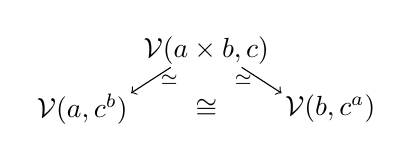
\begin{tikzpicture}[x=1.6em,y=1.5em]
  \node (t)  at (2.8,1.4) {$\mathcal{V}(a\times b,c)$};
  \node (bl) at (0,0)   {$\mathcal{V}(a,c^{b})$};
  \node (br) at (5.6,0) {$\mathcal{V}(b,c^{a})$};
  \draw[->] (2.0,1.0) -- node[right]{$\scriptstyle\simeq$} (1.1,0.38);
  \draw[->] (3.6,1.0) -- node[left]{$\scriptstyle\simeq$} (4.5,0.38);
  \node at (2.8,0) {$\cong$};
\end{tikzpicture}
\end{rveq}
\end{lemma}

\begin{proof}
诸\trFunctor{} $(-)^{a}\colon\mathcal{V}\to\mathcal{V}$ 之族以一种唯一的方式
扩张为\trBifunctor
\[ (-)^{-}\colon\mathcal{V}^{\mathrm{op}}\times\mathcal{V}\to\mathcal{V} \]
使得定义每个\trAdjunction{} $a\times-\dashv(-)^{a}$ 的那些同构
\[ \mathcal{V}(a\times b,c)\cong\mathcal{V}(b,c^{a}) \]
在 $a$ 上（同样也在 $b$ 与 $c$ 上）成为自然的。细节留作%
\cref{ex:extend-to-bifunctors}（或见 \cite[4.3.6]{bib104}）。这就定义了
\eqref{eq:two-variable-adjunction-isos} 右侧的那个自然\trIsomorphism。左侧的
自然\trIsomorphism{}则由与对称\trIsomorphism{} $a\times b\cong b\times a$ 作
复合而定义。第三个自然\trIsomorphism{}取为这两者的复合。
\end{proof}

\begin{example}[\trCartesianClosed{}\trCategory]\label{exa:cartesian-closed-examples}
\begin{enumerate}[label=(\roman*)]
\item 集合的\trCategory{}是\trCartesianClosed，其中 $B^{A}$ 定义为从 $A$
  到 $B$ 的函数之集。跨越自然\trIsomorphism{}
  \eqref{eq:two-variable-adjunction-isos} 的转置被称为「柯里化」（currying）。
\item 小\footnote{一般地，其态射之集被某个固定的不可达基数所界定的诸%
\trCategory{}所组成的\trCategory，在该 Grothendieck 宇宙中是%
\trCartesianClosed{}。}\trCategory{}的\trCategory{} $\Cat$ 是%
\trCartesianClosed{}，其中 $B^{A}$ 定义为从 $A$ 到 $B$ 的诸\trFunctor{}与诸%
\trNaturalTransformation{}的\trCategory。
\[ \Cat(A,C^{B})\cong\Cat(A\times B,C)\cong\Cat(B,C^{A}) \]
上式把诸\trNaturalTransformation{}——即函子\trCategory{}中的箭头
$2\to C^{A}$——与「有向同伦」$A\times 2\to C$ 等同起来。
\item 对任何小\trCategory{} $\mathcal{C}$，\trCategory{}
  $\mathcal{S}et^{\mathcal{C}^{\mathrm{op}}}$ 是\trCartesianClosed。由%
\trYonedaLemma，对 $F,G\in\mathcal{S}et^{\mathcal{C}^{\mathrm{op}}}$，$G^{F}$
在 $c\in\mathcal{C}$ 处的取值必须经由
\[ G^{F}(c)\cong\mathcal{S}et^{\mathcal{C}^{\mathrm{op}}}(\mathcal{C}(-,c),G^{F})
   \cong\mathcal{S}et^{\mathcal{C}^{\mathrm{op}}}(F\times\mathcal{C}(-,c),G) \]
定义为诸\trNaturalTransformation{} $F\times\mathcal{C}(-,c)\Rightarrow G$ 之
集。依照\cref{lem:two-variable-adjunction}，$G^{F}$ 在一个态射
$f\colon c\to c'\in\mathcal{C}$ 上的作用由与相应的\trNaturalTransformation{}
$f\circ-\colon\mathcal{C}(-,c)\Rightarrow\mathcal{C}(-,c')$ 作\trPreComposition{}来定义。
这就定义了\trFunctor{} $G^{F}$。由于任何\trFunctor{}
$H\in\mathcal{S}et^{\mathcal{C}^{\mathrm{op}}}$ 都典范地是诸可表示对象的一个%
\trColimit，这一定义扩充为所需的自然\trIsomorphism{}
$\mathcal{S}et^{\mathcal{C}^{\mathrm{op}}}(H,G^{F})\cong\mathcal{S}et^{\mathcal{C}^{\mathrm{op}}}(F\times H,G)$。
\item 特别地，取 $\mathcal{C}=\boldsymbol{\Delta}$，单纯集的\trCategory{}
  $\sSet:=\mathcal{S}et^{\boldsymbol{\Delta}^{\mathrm{op}}}$ 是%
\trCartesianClosed{}。
\end{enumerate}
\end{example}

指数 $b^{a}$ 常被称为一个\emph{\trInternalHom}（internal hom）。正如这个名称
所暗示的，\trInternalHom{} $b^{a}$ 可以视为 hom-集 $\mathcal{V}(a,b)$ 沿一个
我们即将引入的\trFunctor{}的\trLifting。

\begin{definition}\label{def:underlying-set-functor}
对任何\trCartesianClosed{}\trCategory{} $\mathcal{V}$，\textbf{底集函子}
（underlying set functor）是\trFunctor
\[ \mathcal{V}\xrightarrow{\ (-)_{0}\coloneqq\mathcal{V}(1,-)\ }\mathcal{S}et \]
它由\trTerminal{}对象 $1\in\mathcal{V}$ 所表示。
\end{definition}

\begin{lemma}\label{lem:underlying-set-of-internal-hom}
在一个\trCartesianClosed{}\trCategory{}中，对任何一对对象
$a,b\in\mathcal{V}$，\trInternalHom{} $b^{a}$ 的底集是 $\mathcal{V}(a,b)$，
亦即：
\[ (b^{a})_{0}\cong\mathcal{V}(a,b). \]
\end{lemma}

\begin{proof}
将\cref{def:underlying-set-functor}与
\eqref{eq:two-variable-adjunction-isos} 相结合：
\[ (b^{a})_{0}:=\mathcal{V}(1,b^{a})\cong\mathcal{V}(1\times a,b)
   \cong\mathcal{V}(a,b) \]
这是因为存在自然\trIsomorphism{} $1\times a\cong a$。
\end{proof}

自然会问：底集之间的一个\trIsomorphism{}能否被「富集」而居于 $\mathcal{V}$
之中——亦即，沿底集函子 $(-)_{0}\colon\mathcal{V}\to\mathcal{S}et$ 而被提升？

\begin{lemma}\label{lem:isos-lift-to-V}
一个\trCartesianClosed{}\trCategory{}的定义性双变量\trAdjunction{}所刻画的诸
自然\trIsomorphism{} \eqref{eq:two-variable-adjunction-isos} 提升至
$\mathcal{V}$：对任何 $a,b,c\in\mathcal{V}$，
\begin{rveq}\label{eq:associativity-triangle-isos}
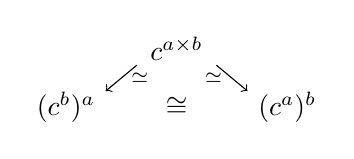
\begin{tikzpicture}[x=1.6em,y=1.5em]
  \node (t)  at (2.5,1.4) {$c^{a\times b}$};
  \node (bl) at (0,0)   {$(c^{b})^{a}$};
  \node (br) at (5.0,0) {$(c^{a})^{b}$};
  \draw[->] (1.6,1.0) -- node[right]{$\scriptstyle\simeq$} (0.9,0.38);
  \draw[->] (3.4,1.0) -- node[left]{$\scriptstyle\simeq$} (4.1,0.38);
  \node at (2.5,0) {$\cong$};
\end{tikzpicture}
\end{rveq}
\end{lemma}

\begin{proof}
这由\cref{lem:two-variable-adjunction}、有限\trProduct{}的结合律以及%
\trYonedaLemma{}推得。为证 \eqref{eq:associativity-triangle-isos}，只需证明
$c^{a\times b}$、$(c^{b})^{a}$ 与 $(c^{a})^{b}$ 表示同一个\trFunctor。通过复合
自然\trIsomorphism{}序列
\begin{align*}
\mathcal{V}(x,(c^{b})^{a})
  &\cong\mathcal{V}(x\times a,c^{b})
    \cong\mathcal{V}((x\times a)\times b,c)
    \cong\mathcal{V}(x\times(a\times b),c)\\
  &\cong\mathcal{V}(x,c^{a\times b})\\
  &\cong\mathcal{V}((a\times b)\times x,c)
    \cong\mathcal{V}(a\times(b\times x),c)
    \cong\mathcal{V}(b\times x,c^{a})\\
  &\cong\mathcal{V}(x,(c^{a})^{b}),
\end{align*}
我们看到
\[ \mathcal{V}(x,(c^{b})^{a})\cong\mathcal{V}(x,c^{a\times b})
   \cong\mathcal{V}(x,(c^{a})^{b}). \]
\end{proof}

\begin{remark}\label{rem:exponent-one-identity}
注意 $(-)^{1}\colon\mathcal{V}\to\mathcal{V}$ 自然\trIsomorphism{}于恒等%
\trFunctor{}——即 $b^{1}\cong b$——因为它是\trFunctor{}
$-\times1\colon\mathcal{V}\to\mathcal{V}$ 的\trRightAdjoint，而后一\trFunctor{}%
自然\trIsomorphism{}于恒等。
\end{remark}

一个\trComplete{}且\trCocomplete{}的\trCartesianClosed{}\trCategory{}是%
\trComplete{}且\trCocomplete{}的封闭对称\trMonoidalCategory{}的一个特例——后者
被 Jean Bénabou 称为一个\textbf{宇宙}（cosmos），以表明这样的基是%
\trEnrichedCategory{}理论的理想环境。出于显然的理由，我们在这里将不使用这个
术语，而是代之以「\trComplete{}且\trCocomplete{}的\trCartesianClosed{}\trCategory」
的说法，以凸显\cref{exa:cartesian-closed-examples}中出现的那些\trCategory{}的
某些共同特征。\footnote{Street \cite{bib117} 曾提出一个与之相竞争的、2-范畴论
意义下的\trFibered{}「宇宙」概念，它与我们所考虑的这个概念更为相近；第 1 章
中的\cref{def:infinity-cosmos}所引入的术语正是直接受其启发。}

\subsection*{练习}

\begin{exercise}\label{ex:extend-to-bifunctors}
证明：在一个\trCartesianClosed{}\trCategory{} $\mathcal{V}$ 中，诸\trFunctor{}
$(-)^{a}\colon\mathcal{V}\to\mathcal{V}$ 之族以一种唯一的方式扩张为\trBifunctor
\[ (-)^{-}\colon\mathcal{V}^{\mathrm{op}}\times\mathcal{V}\to\mathcal{V} \]
使得定义每个\trAdjunction{} $a\times-\dashv(-)^{a}$ 的那个同构
\[ \mathcal{V}(a\times b,c)\cong\mathcal{V}(b,c^{a}) \]
在 $a$ 上（同样也在 $b$ 与 $c$ 上）成为自然的。
\end{exercise}

\begin{exercise}\label{ex:closed-symmetric-monoidal}
一个\textbf{封闭对称幺半范畴}（closed symmetric monoidal category）的数据经由
下述方式推广\cref{def:cartesian-closed}：把有限\trProduct{}换成一个任意的%
\trBifunctor{} $-\otimes-\colon\mathcal{V}\times\mathcal{V}\to\mathcal{V}$，把%
\trTerminal{}对象换成一个对象 $I\in\mathcal{V}$，并额外要求指定诸自然%
\trIsomorphism
\[
a\otimes(b\otimes c)\mathrel{\underset{\alpha}{\cong}}(a\otimes b)\otimes c
\qquad
I\otimes a\mathrel{\underset{\lambda}{\cong}}a
\mathrel{\underset{\rho}{\cong}}a\otimes I
\qquad
a\otimes b\mathrel{\underset{\gamma}{\cong}}b\otimes a
\]
其满足种种相干公理 \cite{bib41,bib66}（另见 \cite{bib69}）。请在%
\trCartesianClosed{}\trCategory{}这一特殊情形下给出这些\trIsomorphism{}的一个%
\trCanonical{}构造，并解释为什么诸相干条件是自动成立的。
\end{exercise}

